\documentclass[12pt]{article}
\usepackage[portuguese]{babel}
\usepackage{fontspec}
\setmainfont{Times New Roman}
\usepackage{amsmath}
\usepackage{amsmath}
\usepackage{amssymb}
\usepackage{graphicx}
\usepackage{natbib}
\usepackage{cite} 
\usepackage{float}
\usepackage{calrsfs}
\usepackage[a4paper,left=2.5cm,right=2.5cm,top=2.5cm, bottom=2.5cm]{geometry}
\usepackage{verbatim}
\usepackage{bigints}
\usepackage{booktabs}
\usepackage[table]{xcolor}
\usepackage{siunitx}
\usepackage{amsfonts}
\usepackage{amssymb}
\usepackage{makeidx}
\usepackage{xcolor}
\usepackage[stable]{footmisc}
\usepackage[section]{placeins}
\usepackage{tabularx}
\usepackage{titlesec}
\usepackage{enumitem}
\titleformat*{\section}{\bfseries\large}
\titleformat*{\subsection}{\bfseries\normalsize}


\usepackage[margin=10pt,labelfont=bf]{caption}


%======================================================================

\begin{document}
\thispagestyle{empty}
\begin{center}
\vspace{0.2cm}

\hrulefill

UNIVERSIDADE FEDERAL DE ALAGOAS\\
PRÓ-REITORIA DE PESQUISA E PÓS-GRADUAÇÃO\\
COORDENADORIA DE PESQUISA

\hrulefill

\vspace{0.5cm}

PROGRAMA INSTITUCIONAL DE BOLSAS DE INICIAÇÃO CIENTÍFICA\\PIBIC/UFAL/FAPEAL/CNPq

\vspace{1.0cm}

\textbf{\Large{RELATÓRIO PARCIAL (2018 -- 2019)}}\\

\end{center}

\vspace{1.2cm}

\textbf{TÍTULO DO PROJETO DE PESQUISA:}

\underline{Análise de Sinais e Imagens com Distâncias Estocásticas e Diferenças de Entropias}

\textbf{TÍTULO DO PLANO DE TRABALHO:}

\underline{Aplicacões Inovadoras da Teoria da Informacão no Processamento e Análise de Imagens e Sinais}

\vspace{1cm}

\begin{table}[!h]
\begin{center}
\begin{tabularx}{\textwidth}{|X|X|X|}
\hline                              
\textbf{Nome Orientador/Unidade/Campus/Email} &  Alejandro C. Frery/Instituto de Computação/Campus A. C. Simões/acfrery@gmail.com\\
\hline     
\textbf{Nome Bolsista ou Colaborador} & Marcos Gleysson Silva do Nascimento\\
\hline     
\textbf{Email/Fones} & mgsn@laccan.ufal.br/(82) 99671-0608\\
\hline     
\end{tabularx}
\end{center}
\end{table}

\begin{table}[!h]
\begin{center}
\begin{tabularx}{\textwidth}{|X|X|X|X|}
\hline                              
X & Bolsista CNPq &  & Bolsista FAPEAL\\
\hline             
& Bolsista UFAL &  & Colaborador\\
\hline             
& Bolsista PIBIC-Af &  &\\
\hline     
\end{tabularx}
\end{center}
\end{table}

\hrulefill   

%=================================================================

\newpage
\section*{\centering \textbf{RESUMO DO PROJETO}}

\vspace{0.2cm}

Houve um significativo avanço nos ultimos anos na obtenção de novos métodos para a extração de informação a partir de sinais e imagens empregando técnicas oriundas da Teoria da Informação. Essas técnicas empregam duas abordagens. A primeira consiste em calcular diversas formas de entropia através de modelos analíticos; essas entropias sao atributos descritores, e podem ser usados para calcular o contraste entre dos sinais, isto é, quão diferentes eles são. A segunda abordagem emprega dois sinais e seus modelos analíticos, e calcula diversas medidas de dissimilaridade entre eles. Tanto os contrastes oriundos de diferenças de entropias quanto as medidas de dissimilaridade podem ser transformados em testes estatísticos com propriedades assintóticas conhecidas tornando-se, assim, poderosas ferramentas para a realização de comparações e para a tomada de decisões. Este projeto irá concentrar-se na aplicacão dessas ferramentas em problemas relevantes de processamento e analise de sinais e imagens. Os principais problemas a serem abordados são na área de processamento e análise de imagens, em particular de imagens de radar de abertura sintetica polarimétrico (SAR -- Synthetic Aperture Radar e PolSAR -- Polarimetric
Synthetic Aperture Radar) e de series temporais. Faremos a proposta de novos filtros, classificadores, segmentadores e detetores de mudança para as primeiras, e de novos descritores e quantificadores de mudança para as segundas. Este projeto irá ainda fazer avanços teóricos. Os resultados conhecidos para os testes estatísticos são válidos apenas no sentido assintótico e quando são empregados estimadores de máxima ´
verossimilhança. Estudaremos extensoes para os casos de amostras finitas e outros tipos de estimadores (baseados no princípio da analogia, robustos, e não-paramétricos, dentre outros).


\textbf{Palavras-chave: Teoria da Informação; Imagens SAR; Séries Temporais} 


%=========================================================
\newpage
\section*{\centering \textbf{OBJETIVOS DO PROJETO DE PESQUISA}}

\vspace{0.5cm}

O objetivo geral deste projeto e avançar a fronteira do conhecimento em duas frentes: análise de dados SAR e de series temporais. A primeira frente segue uma abordagem paramétrica, enquanto a segunda obedece diretrizes nao paramétricas. Ambas têm como suporte conceitual o uso de Teoria da Informação e de Geometria da Informacão para alcançar os objetivos específicos.

O objetivo específico central da primeira frente de trabalho é o desenvolvimento de métodos de estimação do parâmetro que indexa a distribuição $G^{0}$ para modelar dados SAR. Em particular, almejamos alcançar as seguintes metas:

\begin{itemize}
    \item Estudar e implementar técnicas de estimação por momentos fracionários, log-momentos, máxima verossimilhança, máxima verossimilhança iterada, métodos kernel e robustos, além de técnicas para melhorar as estimativas (bootstrap e correções analíticas).
    \item Integrar essas tecnicas em um método unificado que seja capaz de aplicar as mais adequadas para cada caso com a mínima intervenção possível por parte do usuário utilizando a plataforma R.
\end{itemize}

Já que no que diz respeito à segunda frente de trabalho, almejamos desenvolver uma plataforma unificada de analise de séries temporais com métodos de simbolização. Daremos ênfase ao problema da imputação de padrões ausentes, tendo as seguintes metas em vista:

\begin{itemize}
    \item Estudar e implementar técnicas para imputação de padrões ausentes ocasionados por dados repetidos.
    \item Analisar a capacidade de reconstrução de informações dessas técnicas quando a série temporal é armazenada com menos precisão do que a ideal. 
    \item Analisar a distribuição temporal dos padrões originais e imputados.
    \item Desenvolver uma ferramenta para análise de séries temporais baseada em padrões ordinais utilizando a linguagem R.
\end{itemize}

Parte fundamental deste projeto é a verificação das propriedades numéricas do software desenvolvido. Estas propriedades são fundamentais para a aplicação dessas ferramentas na análise de dados. 


%=========================================================
\newpage
\section*{\centering \textbf{OBJETIVO ESPECÍFICO DO TRABALHO DO ALUNO}}

\vspace{0.5cm}

Os objetivos específicos desta frente de trabalho consistem em desenvolver métodos de estimação do parâmetro que indexa a distribuição $G^{0}$ para modelar dados SAR. Estudar e implementar técnicas de estimação por momentos fracionários, log-momentos, máxima verossimilhança, máxima verossimilhança iterada, métodos kernel e robustos, além de técnicas para melhorar as estimativas (bootstrap e correções analíticas). 

Além disso, também faz parte dos objetivos integrar essas técnicas em um método unificado que seja capaz de aplicar as mais adequadas para cada caso com a mínima intervenção possível por parte do usuário utilizando a plataforma R.
%=========================================================

\newpage
\section*{\centering \textbf{ETAPAS DO PLANO DE TRABALHO}}

\vspace{0.5cm}

O presente plano de trabalho tem por título a Estimação do Parâmetro da Lei $G^{0}$. Assim, as etapas necessárias para executar as metas com êxito e alcançar os objetivos propostos neste plano de trabalho são compostas por diversas atividades que vão desde a busca de materiais (artigos, livros, revistas, entre outros) relacionados à temática do projeto até a aplicação dos conhecimentos adquiridos na implementação de \textit{scripts} utilizando a plataforma \texttt{R}. 

Para o início do plano de trabalho que tem por finalidade a implementação de um conjunto de métodos ou rotinas de estimação do parâmetro que indexa a distribuição $G^{0}$ foram exploradas diversas referências de qualidade para que fosse construída uma boa base de conhecimento com a finalidade de prover o devido suporte às realizações dos objetivos finais do projeto.

Todo trabalho científico inicia com uma pergunta científica e, consequentemente, temos um problema a ser analisado e investigado. Nesse sentido, a metodologia correspondente a este plano de trabalho consiste em estudar artigos científicos de bom nível, bem como livros que possam servir de guia, desenvolver protótipos e avaliar seu desempenho com conjuntos de dados de propriedades conhecidas. Além disso, as técnicas e implementações consideradas mais adequadas serão integradas em um sistema de produção de uso facilitado para pesquisadores. 

Após a realização de estudos desenvolvidos a cerca da distribuição $G_I^0$ que trabalha com dados SAR em intensidade, foram estudados os conceitos que permeiam a estatística inferencial que consiste de uma área da Estatística que se utiliza de uma amostra aleatória dos dados coletados de uma população para descrever e fazer inferências sobre a população. As estatísticas inferenciais são valiosas quando não é conveniente ou possível examinar cada membro de uma população por inteiro.

Nesse contexto, para iniciar a pesquisa foi estabelecido o foco em duas técnicas de estimação: Máxima Verossimilhança e Momentos. Nessa etapa, foram estudados os conceitos, fundamentos e as ideias que envolvem cada uma, além de estabelecer as restrições e limites inerentes a aplicação de cada método no contexto da estimação de parâmetros de distribuições de probabilidade. Após o estudo teórico de ambas as técnicas, partiu-se para a implementação das mesmas na plataforma \texttt{R}. A partir desse estudo inicial, a pesquisa evoluiu até o estudo das demais técnicas planejadas para serem estudadas e implementadas. Durante todo esse período de execução da pesquisa a utilização da plataforma \texttt{R} foi bastante frequente.


%=========================================================

\newpage
\section*{\centering \textbf{APRESENTAÇÃO E DISCUSSÃO DOS PRINCIPAIS RESULTADOS}}
\vspace{0.5cm}

Durante a execução do presente projeto de pesquisa, mais especificamente do plano de trabalho relativo a esse relatório, ocorreram resultados bastante positivos relativos aos conceitos e teorias estudadas, bem como às implementações de código desenvolvidas na plataforma \texttt{R}. 

Segundo \citet{FreryStochasticDistances2015}, o modelo $G_I^0$ é indexado por três parâmetros: o número de $Looks$ ($L$) que pode ser estimado em toda a imagem, um parâmetro de escala ($\gamma$) e o parâmetro de rugosidade ou textura ($\alpha$). Uma das características mais importantes da distribuição $G_I^0$ é a interpretação de seu parâmetro $\alpha$ que está relacionado com a rugosidade do alvo. Valores próximos de $0$ (tipicamente acima de $-3$) sugerem alvos extremamente texturizados, como zonas urbanas. Em situações intermediárias, à medida que o valor diminui, isso indica regiões com textura moderada (geralmente $\alpha \in  [−6, −3]$), tipicamente áreas irregulares, como zonas florestais. Alvos sem textura, geralmente produzem $\alpha \in (−\infty, −6)$ como é o caso de regiões lisas, por exemplo, pastagem, culturas e campos queimados. Esta é a razão pela qual a precisão na estimativa de $\alpha$ é tão importante.

Ao longo do primeiro semestre de pesquisa foram implementados em \texttt{R} protótipos das técnicas de estimação estudadas: Máxima Verossimilhança, Método dos Momentos, Método de Log-Cumulantes e Estimação pela Minimização de Distâncias Estocásticas (especificamente da Distância Triangular). Após a implementação, foram realizados testes de unidade a partir de um conjunto de dados com propriedades previamente conhecidas onde se constatou a corretude do algoritmo implementado perante análise do comportamento de entrada e saída do mesmo.

Além disso, foi feito também um experimento de Monte Carlo que de acordo com \citet{busto92}, experiências de Monte Carlo são uma poderosa técnica estatística usada para fornecer respostas aproximadas para questões sobre problemas complexos que podem incluir um componente estocástico, principalmente quando as técnicas analíticas e numéricas não fornecem, com uma quantidade aceitável de esforço, essas respostas de forma exata e completa. Estas técnicas de simulação são essencialmente baseadas em amostragem estatística controlada, e elas têm uma ampla gama de aplicações, incluindo, entre outras, mecânica estatística, biologia, jogos, otimização combinatória e engenharia.

Nesse contexto, um experimento de Monte Carlo foi definido para avaliar o desempenho de cada técnica de estimação definidas acima no cálculo dos estimadores. O espaço de parâmetros utilizado consiste na grade formada pela tabela a seguir onde variou-se o parâmetro de textura $\alpha$ de modo a englobar a simulação de regiões extremamente texturizadas, de textura moderada e alvos sem textura. O parâmetro $n$, número de amostras, também foi variado de forma a representar amostras consideravelmente pequenas, médias e grandes. O parâmetros $Looks$ teve seu valor constante no experimento. Vale ressaltar que o valor de $\gamma*$ foi dado em função do parâmetro $\alpha$ de modo a simplificar os cálculos de geração dos estimadores.
\begin{table}[H]
\centering
\caption{Espaço de parâmetros utilizado na simulação}
\smallskip
\sisetup{table-format = 3.2}
\label{tab:tabela_parameters}
\begin{tabular}{c|c}
\toprule 
\multicolumn{1}{c|}{Parâmetros} & \multicolumn{1}{c}{Valores}  \\ 
\midrule
\rowcolor[gray]{.9} 
$n$ & \{200, 2000, 10000\} \\ \hline
$\alpha$ & \{-2, -5, -8\} \\ \hline
\rowcolor[gray]{.9} $\gamma*$ & \{-$\alpha$ - 1\} \\ \hline
$Looks$ & \{3\} \\ 
\bottomrule
\end{tabular}
\end{table}

Nesse experimento foi feito um total de 1000 replicações onde 1000 amostras foram geradas para cada ponto do espaço de parâmetros considerado na tabela anterior. Dessa forma, foi produzido o vetor de estimadores, $\{\widehat{\alpha}_{1}, \widehat{\alpha}_{2}, \dots, \widehat{\alpha}_{1000} \}$. Com esse vetor em mãos, foram então calculados para cada caso a média das mil estimativas, $ \overline{\widehat{\alpha}} = (1000)^{-1} \sum_{i=1}^{1000} \widehat{\alpha_{i}} $. Abaixo encontra-se uma tabela com os resultados dos estimadores de Máxima Verossimilhança para o parâmetro $\alpha$ da $G_I^0$.
\begin{table}[H]
\centering
\caption{Estimadores de Máxima Verossimilhança} 
\begin{tabular}{@{\extracolsep{4pt}}c|c|c|c|c}
\toprule   
\multicolumn{1}{c}{\textbf{Amostras}} & \multicolumn{1}{c}{\textbf{Escala}} & \multicolumn{1}{c}{\textbf{Looks}} & \multicolumn{1}{c}{\textbf{Textura}} & \multicolumn{1}{c}{\textbf{Est. de Max. Ver.}} \\
 \cmidrule{1-1} 
 \cmidrule{2-2} 
 \cmidrule{3-3} 
 \cmidrule{4-4} 
 \cmidrule{5-5} 
\multicolumn{1}{c}{$n$} & \multicolumn{1}{c}{$\gamma$} & \multicolumn{1}{c}{$L$} & \multicolumn{1}{c}{$\alpha$} & \multicolumn{1}{c}{$\widehat{\alpha}_{MV}$} \\ 
\midrule
200  & 1 & 3 & -2 & -1.940  \\ 
   & 4 & ~ & -5 & -5.275  \\ 
   & 7 & ~ & -8 & -9.223  \\ \hline
2000  & 1 & 3 & -2 & -2.001   \\ 
   & 4 & ~ & -5 & -5.027    \\
   & 7 & ~ & -8 & -8.074   \\ \hline
10000  & 1 & 3 & -2 & -2.001  \\ 
   & 4 & ~ & -5 & -5.005   \\
   & 7 & ~ & -8 & -8.015    \\
\bottomrule
\end{tabular}
\end{table}

De modo análogo, abaixo está a tabela que contém os resultados dos estimadores de Momentos encontrados com o procedimento de Monte Carlo definido.
\begin{table}[H]
\centering
\caption{Estimadores de Momentos} 
\begin{tabular}{@{\extracolsep{4pt}}c|c|c|c|c}
\toprule   
\multicolumn{1}{c}{\textbf{Amostras}} & \multicolumn{1}{c}{\textbf{Escala}} & \multicolumn{1}{c}{\textbf{Looks}} & \multicolumn{1}{c}{\textbf{Textura}} & \multicolumn{1}{c}{\textbf{Est. de Momentos}} \\
 \cmidrule{1-1} 
 \cmidrule{2-2} 
 \cmidrule{3-3} 
 \cmidrule{4-4} 
 \cmidrule{5-5} 
\multicolumn{1}{c}{$n$} & \multicolumn{1}{c}{$\gamma$} & \multicolumn{1}{c}{$L$} & \multicolumn{1}{c}{$\alpha$} & \multicolumn{1}{c}{$\widehat{\alpha}_{Mom12}$} \\ 
\midrule
200  & 1 & 3 & -2 & -2.209  \\ 
   & 4 & ~ & -5 & -5.254  \\ 
   & 7 & ~ & -8 & -7.211  \\ \hline
2000  & 1 & 3 & -2 & -2.012   \\ 
   & 4 & ~ & -5 & -5.046    \\
   & 7 & ~ & -8 & -8.172   \\ \hline
10000  & 1 & 3 & -2 & -2.001  \\ 
   & 4 & ~ & -5 & -5.069   \\
   & 7 & ~ & -8 & -8.208    \\
\bottomrule
\end{tabular}
\end{table}

Por usa vez, a seguir encontram-se os estimadores de Log-Cumulantes encontrados a partir do procedimento realizado.
\begin{table}[H]
\centering
\caption{Estimadores de Log-Cumulantes} 
\begin{tabular}{@{\extracolsep{4pt}}c|c|c|c|c}
\toprule   
\multicolumn{1}{c}{\textbf{Amostras}} & \multicolumn{1}{c}{\textbf{Escala}} & \multicolumn{1}{c}{\textbf{Looks}} & \multicolumn{1}{c}{\textbf{Textura}} & \multicolumn{1}{c}{\textbf{Est. Log-Cumulantes}} \\
 \cmidrule{1-1} 
 \cmidrule{2-2} 
 \cmidrule{3-3} 
 \cmidrule{4-4} 
 \cmidrule{5-5} 
\multicolumn{1}{c}{$n$} & \multicolumn{1}{c}{$\gamma$} & \multicolumn{1}{c}{$L$} & \multicolumn{1}{c}{$\alpha$} & \multicolumn{1}{c}{$\widehat{\alpha}_{LCum}$} \\ 
\midrule
200  & 1 & 3 & -2 & -2.027  \\ 
   & 4 & ~ & -5 & -4.972  \\ 
   & 7 & ~ & -8 & -7.908  \\ \hline
2000  & 1 & 3 & -2 & -2.004   \\ 
   & 4 & ~ & -5 & -5.094   \\
   & 7 & ~ & -8 & -8.225   \\ \hline
10000  & 1 & 3 & -2 & -2.000  \\ 
   & 4 & ~ & -5 & -5.008   \\
   & 7 & ~ & -8 & -8.064    \\
\bottomrule
\end{tabular}
\end{table}

Por fim, abaixo, encontram-se os estimadores gerados pela Minimização de Distâncias Estocásticas.
\begin{table}[H]
\centering
\caption{Estimadores de Distâncias Estocásticas} 
\begin{tabular}{@{\extracolsep{4pt}}c|c|c|c|c}
\toprule   
\multicolumn{1}{c}{\textbf{Amostras}} & \multicolumn{1}{c}{\textbf{Escala}} & \multicolumn{1}{c}{\textbf{Looks}} & \multicolumn{1}{c}{\textbf{Textura}} & \multicolumn{1}{c}{\textbf{Est. Distâncias Estocásticas}} \\
 \cmidrule{1-1} 
 \cmidrule{2-2} 
 \cmidrule{3-3} 
 \cmidrule{4-4} 
 \cmidrule{5-5} 
\multicolumn{1}{c}{$n$} & \multicolumn{1}{c}{$\gamma$} & \multicolumn{1}{c}{$L$} & \multicolumn{1}{c}{$\alpha$} & \multicolumn{1}{c}{$\widehat{\alpha}_{DT}$} \\ 
\midrule
200  & 1 & 3 & -2 & -2.037  \\ 
   & 4 & ~ & -5 & -4.372  \\ 
   & 7 & ~ & -8 & -6.865  \\ \hline
2000  & 1 & 3 & -2 & -1.191   \\ 
   & 4 & ~ & -5 & -4.094   \\
   & 7 & ~ & -8 & -6.534   \\ \hline
10000  & 1 & 3 & -2 & -1.194  \\ 
   & 4 & ~ & -5 & -3.076   \\
   & 7 & ~ & -8 & -6.538    \\
\bottomrule
\end{tabular}
\end{table}

A seguir estão os gráficos que mostram uma comparação das estimativas providas pelas técnicas de estimação implementadas neste trabalho: Máxima Verossimilhança, Momentos, Log-Cumulantes e Distâncias Estocásticas.
\begin{figure}[H]
     \centering
     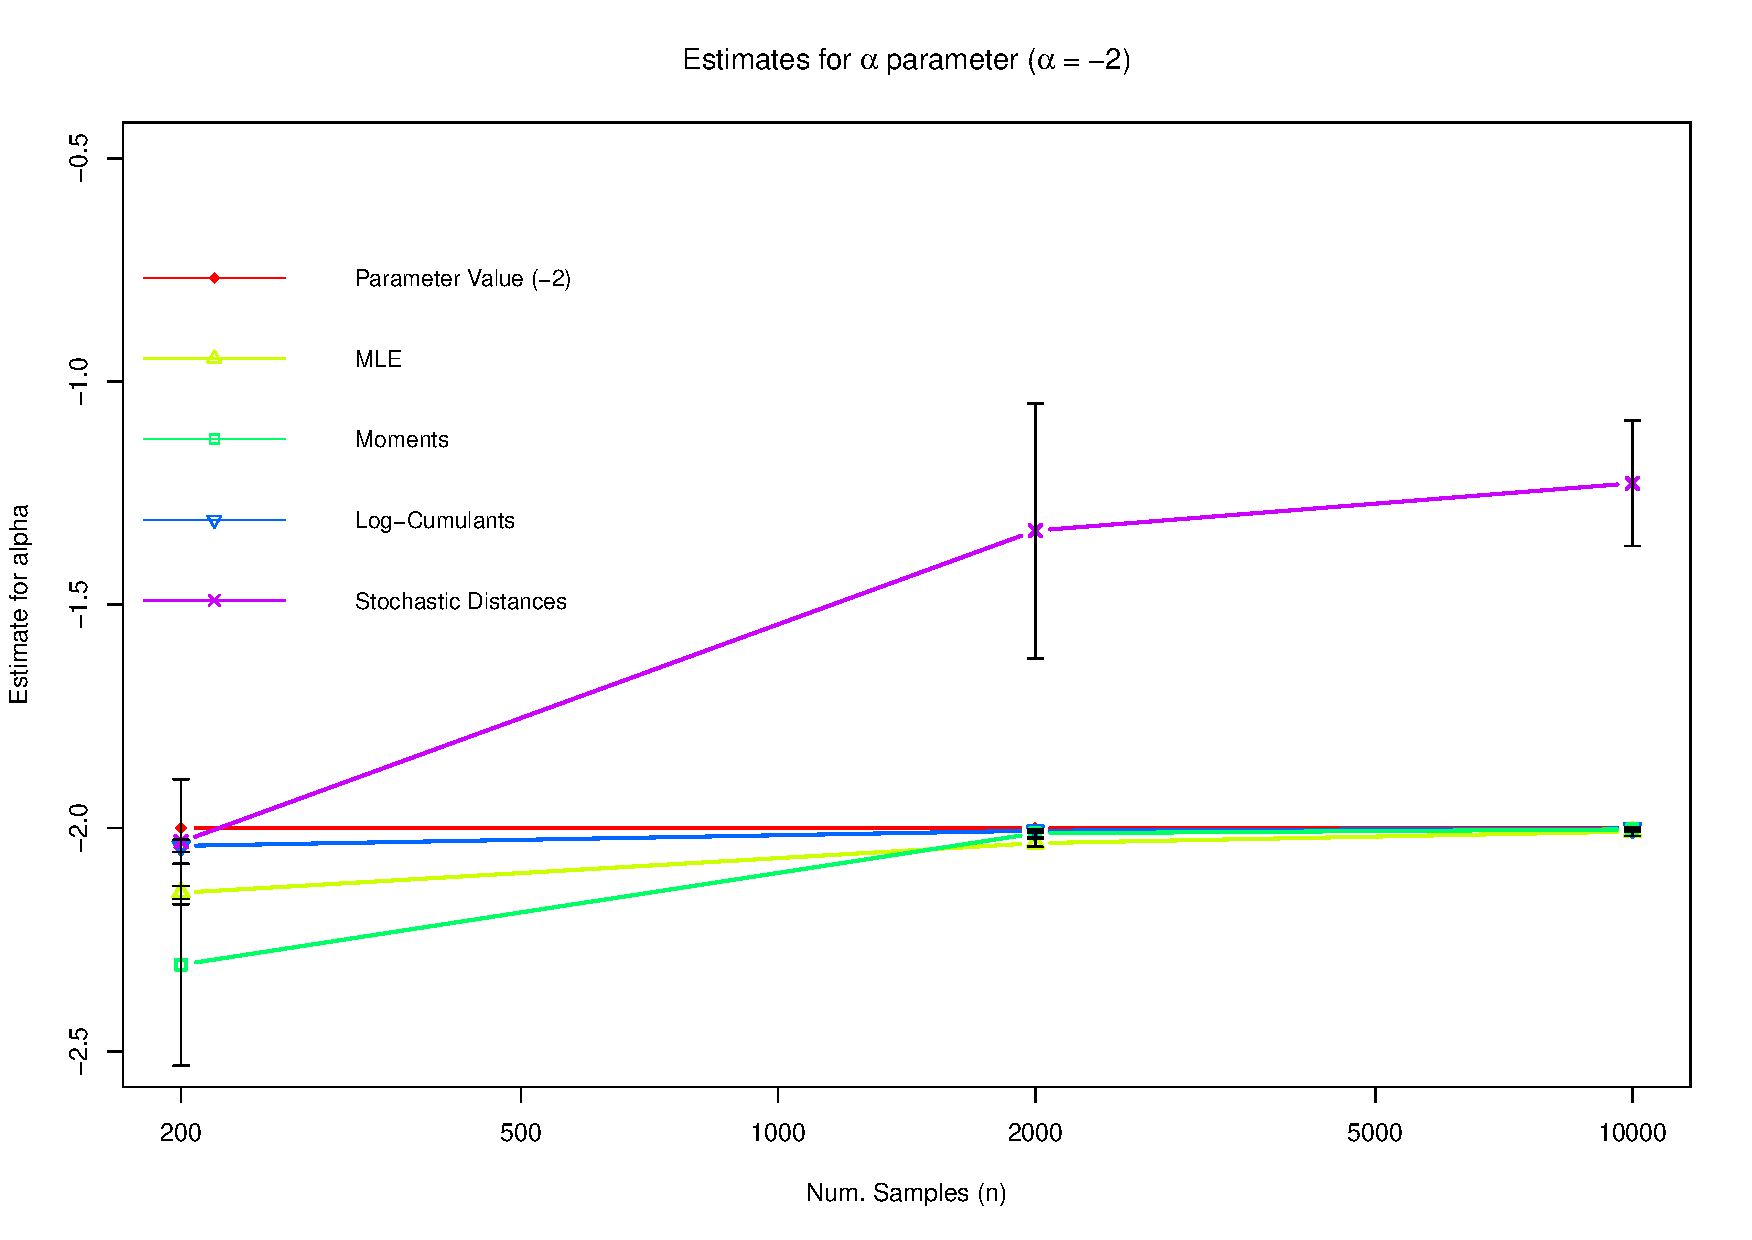
\includegraphics[scale=0.5]{plots/ComparisonAlpha-2.pdf}
     \caption{Estimativas obtidas para o parâmetro $\alpha = -2$}
     \label{graf_5}
\end{figure}
\begin{figure}[H]
     \centering
     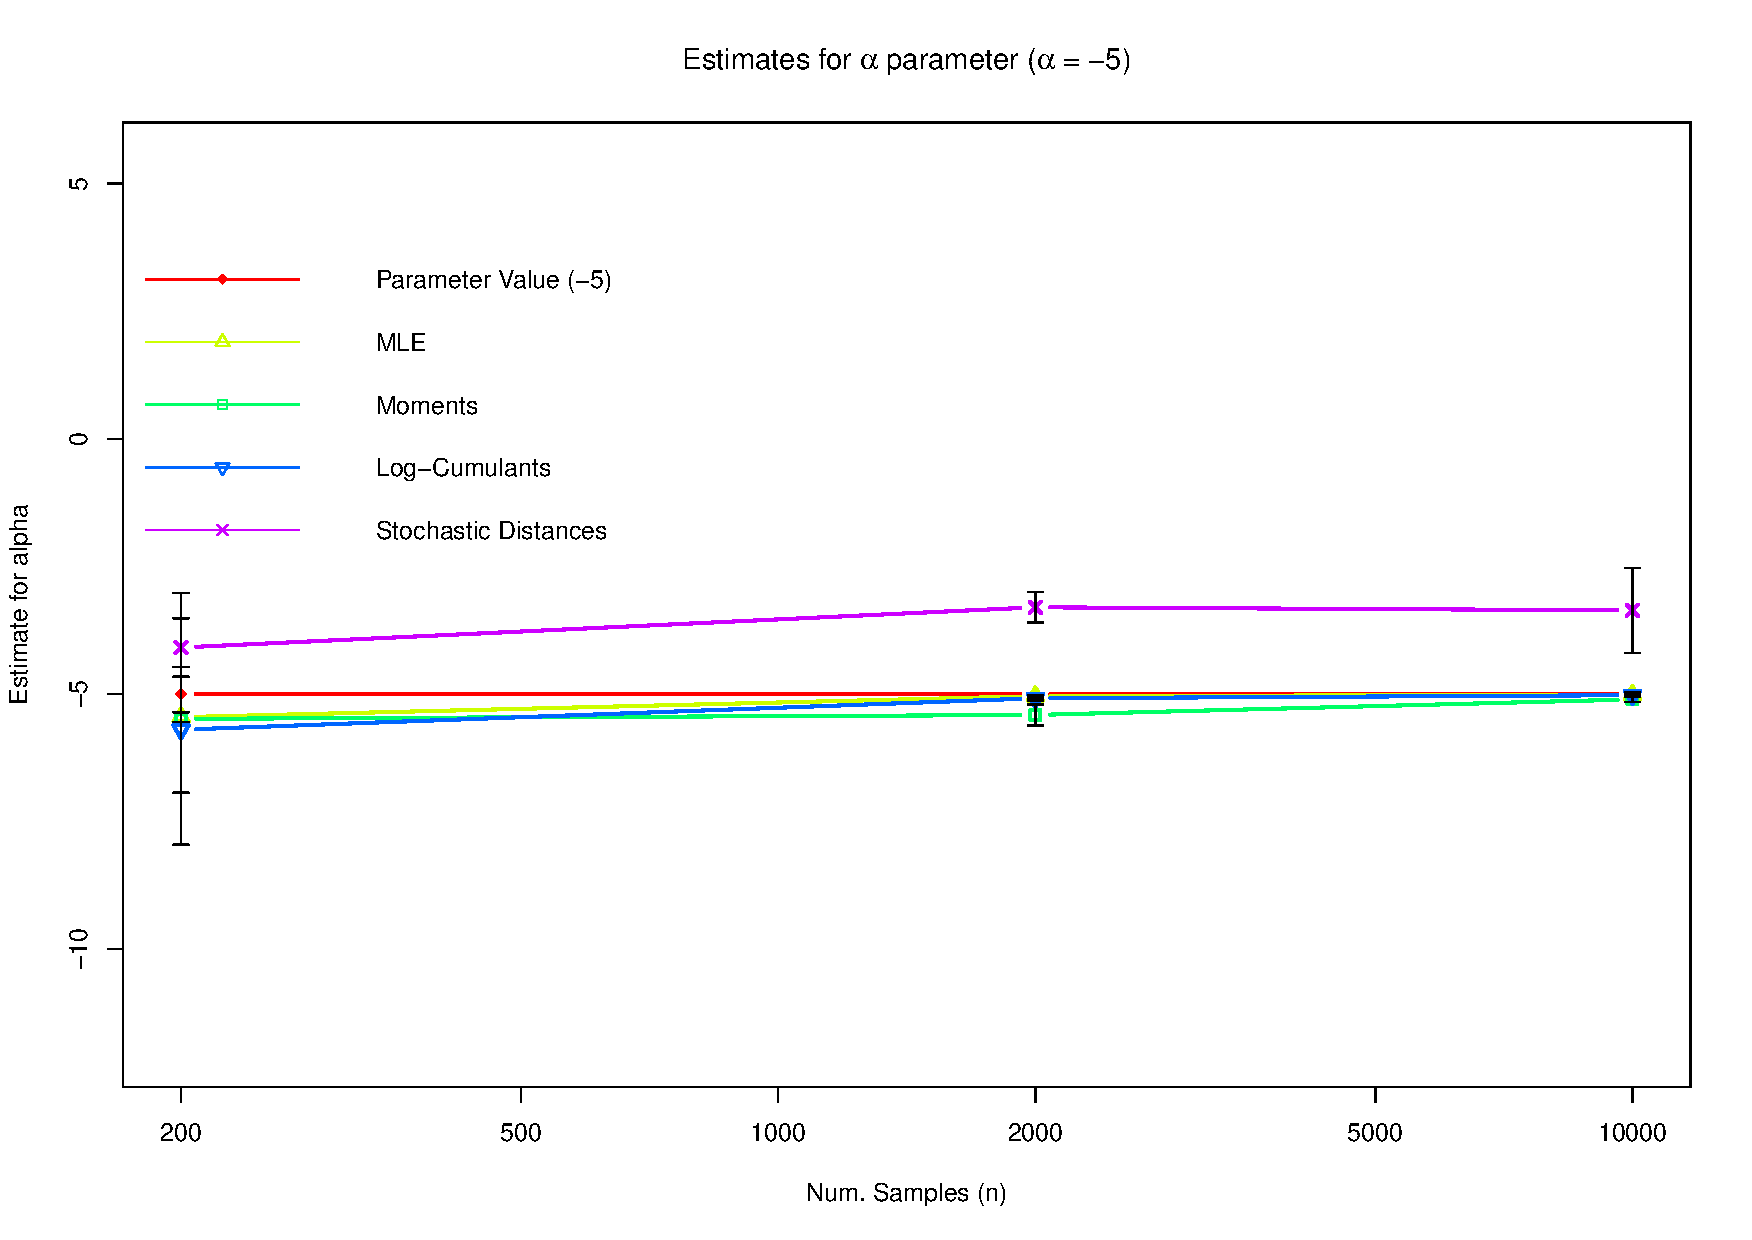
\includegraphics[scale=0.5]{plots/ComparisonAlpha-5.pdf}
     \caption{Estimativas obtidas para o parâmetro $\alpha = -5$}
     \label{graf_6}
\end{figure}
\begin{figure}[H]
     \centering
     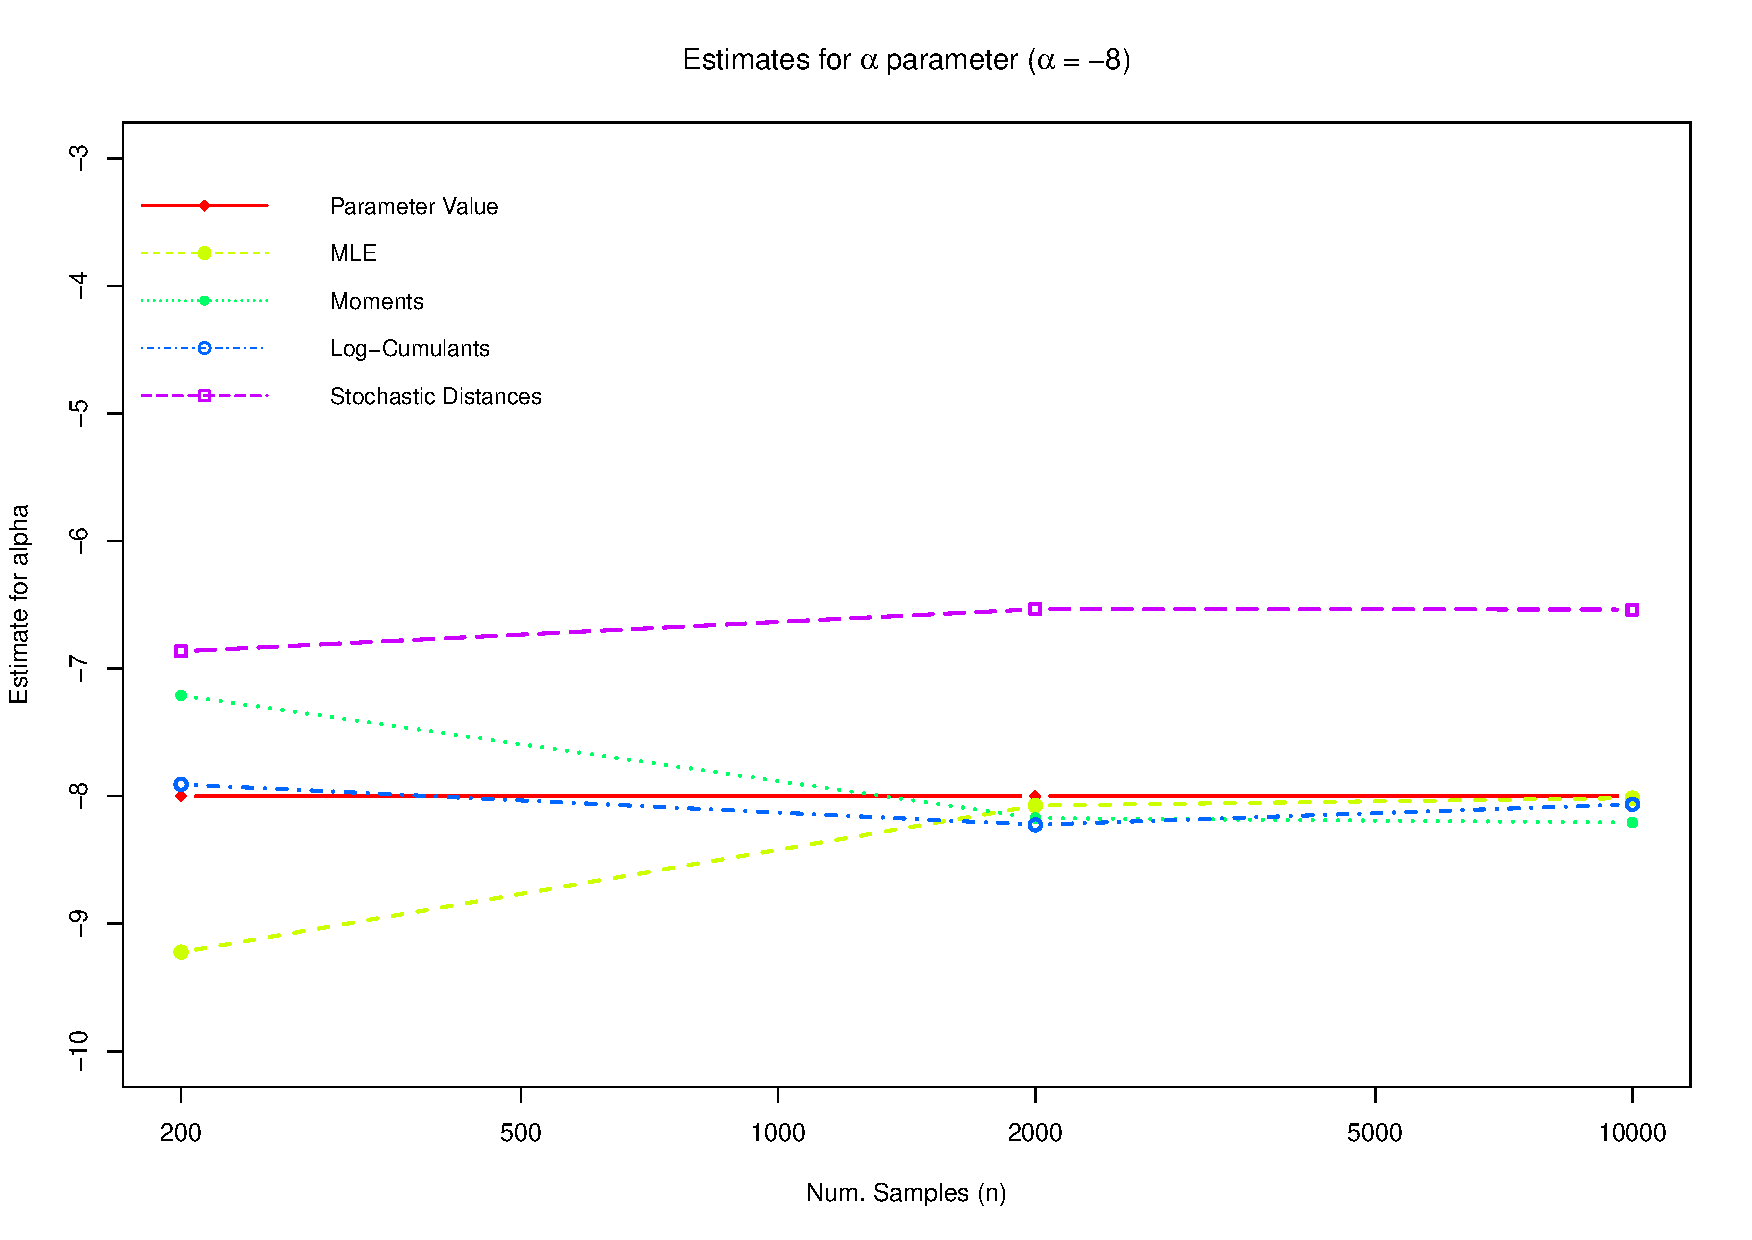
\includegraphics[scale=0.5]{plots/ComparisonAlpha-8.pdf}
     \caption{Estimativas obtidas para o parâmetro $\alpha = -8$}
     \label{graf_7}
\end{figure}

Para o estudo de simulação feito, pode-se perceber através dos gráficos que 3 métodos de estimação conquistaram ótimos resultados e que, de certa forma, se mostraram semelhantes entre si. Tais métodos foram os baseados em Máxima Verossimilhança, Momentos e Log-Momentos e estes apresentaram convergência para o verdadeiro valor do parâmetro na maioria dos casos testados. O estimador baseado em mecanismos da Teoria da Informação, mas especificamente na Minimização de Distâncias Estocásticas, foi o que apresentou resultados mais discrepantes em relação aos demais métodos.

Entretanto, este foi apenas um estudo inicial a respeito das técnicas de estimação de parâmetros implementadas e estão sendo feitos novos planos de simulação e investigação para avaliar o desempenho dos métodos de estimação implementados, bem como analisar suas possíveis restrições e aplicações em um contexto unificado, onde existirá uma rotina de estimação geral que engloba esses métodos e seja capaz de aplicar os mais adequados para cada situação com a mínima intervenção possível do usuário tendo em vista seus pontos fortes e fracos de aplicação. 

%=========================================================

\newpage
\section*{\centering \textbf{CRONOGRAMA DE ATIVIDADES}}
\vspace{0.5cm}

As atividades elaboradas e planejadas para o respectivo plano de trabalho estão listadas logo abaixo:

\begin{enumerate} 
  \item  Conhecer técnicas de estimacão de parâmetros, suas limitações, possíveis implementações e aplicacões.
  \item  Aprender o uso da plataforma \texttt{R}
  \item  Conhecer técnicas de projeto e implementação de software científico usando \texttt{R}.
  \item  Estudar e Implementar técnica de estimação por Máxima Verossimilhança
  \item  Estudar e Implementar técnica de estimação por Momentos
  \item  Estudar e Implementar técnica de estimação por Log-Cumulantes ou Log-Momentos
  \item  Estudar e Implementar técnica de estimação por Distâncias Estocásticas
  \item  Aplicar as técnicas desenvolvidas a conjuntos de dados de propriedades conhecidas. 
  \item  Integrar as tecnicas desenvolvidas em uma plataforma de produção
\end{enumerate}

\begin{figure}[!hbt]
	\begin{center}
    \vspace{-0.5cm}
		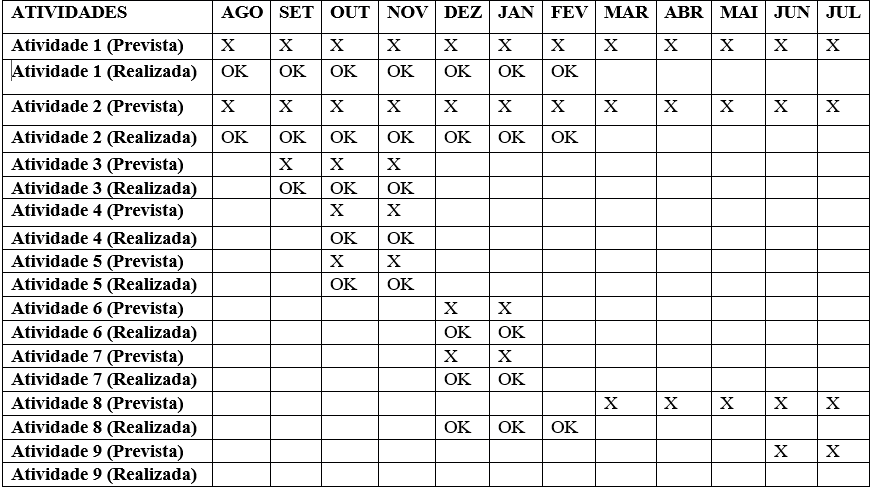
\includegraphics[width=0.9\columnwidth]{tabela-cronograma.png}
	\end{center}
\end{figure}

Este cronograma apresenta algumas modificações em relação ao cronograma inicial proposto no projeto de pesquisa. No cronograma inicial eram propostos 6 meses para o desenvolvimento dos protótipos de algoritmos de estimação. No entanto, com o intuito de adquirir um maior avanço nas pesquisas e um alcance mais rápido de resultados, o escopo foi alterado para comportar apenas 4 meses, em que o tempo ganho iria ser direcionado para análises mais profundas das técnicas implementadas. Assim, chegou-se ao acordo de que iriam ser trabalhadas 4 técnicas (Máxima Verossimilhança, Momentos, Log-Momentos e Distâncias Estocásticas). Consequentemente, a atividade 8 também foi adiantada, visto que os métodos de estimação já estavam implementados e, assim, conjuntos de dados de propriedades conhecidas já foram aplicados às técnicas desenvolvidas a partir do mês de Dezembro. Ademais, o andamento da pesquisa está conforme o esperado e resultados positivos, tanto teóricos quanto práticos, estão sendo obtidos com êxito ao longo do período estipulado para o projeto. 

%=========================================================

\newpage
\section*{\centering \textbf{FATORES POSITIVOS E NEGATIVOS NA CONDUÇÃO DO PROJETO E PLANO DE TRABALHO}}

\vspace{0.5cm}

Podemos citar como fatores positivos o fato de existir muitos materiais de qualidade (livros, artigos, entre outros) referentes ao tema do projeto da pesquisa, bem como o fato de existirem seminários semanalmente no Laboratório de Computação Científica e Análise Numérica (LaCCAN) que geram a aquisição de novos conhecimentos a respeito de diversos temas provenientes dos demais projetos dos demais pesquisadores do laboratório. Além desses fatores positivos, podemos citar também o fato de existirem reuniões frequentes com o orientador em que podem ser mostrados e discutidos os resultados obtidos e novos objetivos podem ser traçados. 

Ademais, com exceção da fase inicial de preparação e leitura de materiais (livros, artigos, etc) para prover o devido engajamento inicial no projeto, até o presente momento da pesquisa não houveram pontos negativos significativos que tenha interferido negativamente no desenvolvimento do projeto. 


%==============================================================================================================

\newpage
\bibliographystyle{agsm}

\bibliography{../../../Bibliography/references}
%\bibliography{references}



\end{document}